\documentclass[twoside]{book}

% Packages required by doxygen
\usepackage{fixltx2e}
\usepackage{calc}
\usepackage{doxygen}
\usepackage[export]{adjustbox} % also loads graphicx
\usepackage{graphicx}
\usepackage[utf8]{inputenc}
\usepackage{makeidx}
\usepackage{multicol}
\usepackage{multirow}
\PassOptionsToPackage{warn}{textcomp}
\usepackage{textcomp}
\usepackage[nointegrals]{wasysym}
\usepackage[table]{xcolor}

% Font selection
\usepackage[T1]{fontenc}
\usepackage[scaled=.90]{helvet}
\usepackage{courier}
\usepackage{amssymb}
\usepackage{sectsty}
\renewcommand{\familydefault}{\sfdefault}
\allsectionsfont{%
  \fontseries{bc}\selectfont%
  \color{darkgray}%
}
\renewcommand{\DoxyLabelFont}{%
  \fontseries{bc}\selectfont%
  \color{darkgray}%
}
\newcommand{\+}{\discretionary{\mbox{\scriptsize$\hookleftarrow$}}{}{}}

% Page & text layout
\usepackage{geometry}
\geometry{%
  a4paper,%
  top=2.5cm,%
  bottom=2.5cm,%
  left=2.5cm,%
  right=2.5cm%
}
\tolerance=750
\hfuzz=15pt
\hbadness=750
\setlength{\emergencystretch}{15pt}
\setlength{\parindent}{0cm}
\setlength{\parskip}{3ex plus 2ex minus 2ex}
\makeatletter
\renewcommand{\paragraph}{%
  \@startsection{paragraph}{4}{0ex}{-1.0ex}{1.0ex}{%
    \normalfont\normalsize\bfseries\SS@parafont%
  }%
}
\renewcommand{\subparagraph}{%
  \@startsection{subparagraph}{5}{0ex}{-1.0ex}{1.0ex}{%
    \normalfont\normalsize\bfseries\SS@subparafont%
  }%
}
\makeatother

% Headers & footers
\usepackage{fancyhdr}
\pagestyle{fancyplain}
\fancyhead[LE]{\fancyplain{}{\bfseries\thepage}}
\fancyhead[CE]{\fancyplain{}{}}
\fancyhead[RE]{\fancyplain{}{\bfseries\leftmark}}
\fancyhead[LO]{\fancyplain{}{\bfseries\rightmark}}
\fancyhead[CO]{\fancyplain{}{}}
\fancyhead[RO]{\fancyplain{}{\bfseries\thepage}}
\fancyfoot[LE]{\fancyplain{}{}}
\fancyfoot[CE]{\fancyplain{}{}}
\fancyfoot[RE]{\fancyplain{}{\bfseries\scriptsize Generated by Doxygen }}
\fancyfoot[LO]{\fancyplain{}{\bfseries\scriptsize Generated by Doxygen }}
\fancyfoot[CO]{\fancyplain{}{}}
\fancyfoot[RO]{\fancyplain{}{}}
\renewcommand{\footrulewidth}{0.4pt}
\renewcommand{\chaptermark}[1]{%
  \markboth{#1}{}%
}
\renewcommand{\sectionmark}[1]{%
  \markright{\thesection\ #1}%
}

% Indices & bibliography
\usepackage{natbib}
\usepackage[titles]{tocloft}
\setcounter{tocdepth}{3}
\setcounter{secnumdepth}{5}
\makeindex

% Hyperlinks (required, but should be loaded last)
\usepackage{ifpdf}
\ifpdf
  \usepackage[pdftex,pagebackref=true]{hyperref}
\else
  \usepackage[ps2pdf,pagebackref=true]{hyperref}
\fi
\hypersetup{%
  colorlinks=true,%
  linkcolor=blue,%
  citecolor=blue,%
  unicode%
}

% Custom commands
\newcommand{\clearemptydoublepage}{%
  \newpage{\pagestyle{empty}\cleardoublepage}%
}

\usepackage{caption}
\captionsetup{labelsep=space,justification=centering,font={bf},singlelinecheck=off,skip=4pt,position=top}

%===== C O N T E N T S =====

\begin{document}

% Titlepage & ToC
\hypersetup{pageanchor=false,
             bookmarksnumbered=true,
             pdfencoding=unicode
            }
\pagenumbering{alph}
\begin{titlepage}
\vspace*{7cm}
\begin{center}%
{\Large Laboratoire 7\+: Tic Tac Toe \\[1ex]\large 0.\+1 }\\
\vspace*{1cm}
{\large Generated by Doxygen 1.8.13}\\
\end{center}
\end{titlepage}
\clearemptydoublepage
\pagenumbering{roman}
\tableofcontents
\clearemptydoublepage
\pagenumbering{arabic}
\hypersetup{pageanchor=true}

%--- Begin generated contents ---
\chapter{Class Index}
\section{Class List}
Here are the classes, structs, unions and interfaces with brief descriptions\+:\begin{DoxyCompactList}
\item\contentsline{section}{\hyperlink{classlab7_1_1TicTacToe}{lab7\+::\+Tic\+Tac\+Toe} }{\pageref{classlab7_1_1TicTacToe}}{}
\end{DoxyCompactList}

\chapter{File Index}
\section{File List}
Here is a list of all documented files with brief descriptions\+:\begin{DoxyCompactList}
\item\contentsline{section}{\hyperlink{TicTacToe_8cpp}{Tic\+Tac\+Toe.\+cpp} }{\pageref{TicTacToe_8cpp}}{}
\item\contentsline{section}{{\bfseries Tic\+Tac\+Toe.\+h} }{\pageref{TicTacToe_8h}}{}
\end{DoxyCompactList}

\chapter{Class Documentation}
\hypertarget{classlab7_1_1TicTacToe}{}\section{lab7\+:\+:Tic\+Tac\+Toe Class Reference}
\label{classlab7_1_1TicTacToe}\index{lab7\+::\+Tic\+Tac\+Toe@{lab7\+::\+Tic\+Tac\+Toe}}


{\ttfamily \#include $<$Tic\+Tac\+Toe.\+h$>$}

\subsection*{Public Member Functions}
\begin{DoxyCompactItemize}
\item 
\hyperlink{classlab7_1_1TicTacToe_aaaee62ac2cc9f9073795ecb3019764f4}{Tic\+Tac\+Toe} ()
\item 
\hyperlink{classlab7_1_1TicTacToe_a192d59b62d1c9a457362125183747604}{Tic\+Tac\+Toe} (const int p\+\_\+en\+Cours\mbox{[}3\mbox{]}\mbox{[}3\mbox{]})
\item 
int \hyperlink{classlab7_1_1TicTacToe_afb556c0c233a8eb48a67cda693ca8caf}{au\+Tour\+De} () const
\item 
bool \hyperlink{classlab7_1_1TicTacToe_abe77507818b76ed4043de6ffdf1c5675}{joue} (int, int)
\item 
bool \hyperlink{classlab7_1_1TicTacToe_abb76ec869ae10c6ce527759fbadacc25}{carre\+Est\+Libre} (const int p\+\_\+rangee, const int p\+\_\+colonne) const
\item 
bool \hyperlink{classlab7_1_1TicTacToe_a8e72e4ebd69642f050c74f2c41adf734}{grille\+Est\+Remplie} () const
\item 
bool \hyperlink{classlab7_1_1TicTacToe_adc4d6d6c61aac80e4cc26b995ce72a86}{rangee\+Est\+Gagnante} (const int p\+\_\+rangee) const
\item 
bool \hyperlink{classlab7_1_1TicTacToe_a802b609bbe8e0614fe2a6a9234c79899}{colonne\+Est\+Gagnante} (const int p\+\_\+colonne) const
\item 
bool \hyperlink{classlab7_1_1TicTacToe_a422b5f693cf88fb002eb3f87187999a4}{diagonale\+Est\+Gagnante} (const bool p\+\_\+diagonale\+Du\+Coin\+Sup\+Gauche) const
\item 
bool \hyperlink{classlab7_1_1TicTacToe_a2bc802f8841b514aa27932a3202f9e1b}{partie\+Est\+Gagnee} () const
\item 
bool \hyperlink{classlab7_1_1TicTacToe_a278f97c96f7c1e646f16532dd0ac21ae}{partie\+Est\+Nulle} () const
\item 
bool \hyperlink{classlab7_1_1TicTacToe_a3480fd52c83f0c3631a5686ea5e51d4e}{partie\+Est\+Terminee} () const
\item 
int \hyperlink{classlab7_1_1TicTacToe_a6b79c847e3f8088602e869fd88cf4479}{req\+Gagnant} () const
\item 
void \hyperlink{classlab7_1_1TicTacToe_a09cc7980d7f465b21880971e5bccf178}{affiche} () const
\item 
std\+::string \hyperlink{classlab7_1_1TicTacToe_ad014f5c637baa564c99d4ddb0e744f8e}{req\+Grille\+Formattee} (const char symboles\mbox{[}3\mbox{]}) const
\end{DoxyCompactItemize}


\subsection{Detailed Description}
Représentation d\textquotesingle{}un jeu de tic-\/tac-\/toe. Contient une grille de 3 x 3 contenant des entiers. Chaque entier peut prendre les valeurs suivantes\+: ~\newline
0\+: case vide~\newline
1\+: coup du joueur 1~\newline
2\+: coup du joeur 2~\newline
 La classe contient aussi les méthodes permettant de garantir la validité de la grille. Le joueur 1 joue toujours en premier et les deux joueurs jouent à tour de rôle de sorte que le nombre de 1 et de 2 doit être égale ou différer de un.

Il y a aussi les méthodes nécessaires pour assurer la bonne marche du jeu\+: vérifier si la partie est gagnée, si la partie est terminée et si la partie est nulle, ainsi qu\textquotesingle{}identifier le joueur gagnant.

Il y a aussi une méthode d\textquotesingle{}IO à la console, permettant une mise en oeuvre rapide. 

\subsection{Constructor \& Destructor Documentation}
\mbox{\Hypertarget{classlab7_1_1TicTacToe_aaaee62ac2cc9f9073795ecb3019764f4}\label{classlab7_1_1TicTacToe_aaaee62ac2cc9f9073795ecb3019764f4}} 
\index{lab7\+::\+Tic\+Tac\+Toe@{lab7\+::\+Tic\+Tac\+Toe}!Tic\+Tac\+Toe@{Tic\+Tac\+Toe}}
\index{Tic\+Tac\+Toe@{Tic\+Tac\+Toe}!lab7\+::\+Tic\+Tac\+Toe@{lab7\+::\+Tic\+Tac\+Toe}}
\subsubsection{\texorpdfstring{Tic\+Tac\+Toe()}{TicTacToe()}\hspace{0.1cm}{\footnotesize\ttfamily [1/2]}}
{\footnotesize\ttfamily lab7\+::\+Tic\+Tac\+Toe\+::\+Tic\+Tac\+Toe (\begin{DoxyParamCaption}{ }\end{DoxyParamCaption})}

Constructeur par défaut\+: construit une grille vide. Provoque un échec d\textquotesingle{}assertion si la grille est non-\/valide \mbox{\Hypertarget{classlab7_1_1TicTacToe_a192d59b62d1c9a457362125183747604}\label{classlab7_1_1TicTacToe_a192d59b62d1c9a457362125183747604}} 
\index{lab7\+::\+Tic\+Tac\+Toe@{lab7\+::\+Tic\+Tac\+Toe}!Tic\+Tac\+Toe@{Tic\+Tac\+Toe}}
\index{Tic\+Tac\+Toe@{Tic\+Tac\+Toe}!lab7\+::\+Tic\+Tac\+Toe@{lab7\+::\+Tic\+Tac\+Toe}}
\subsubsection{\texorpdfstring{Tic\+Tac\+Toe()}{TicTacToe()}\hspace{0.1cm}{\footnotesize\ttfamily [2/2]}}
{\footnotesize\ttfamily lab7\+::\+Tic\+Tac\+Toe\+::\+Tic\+Tac\+Toe (\begin{DoxyParamCaption}\item[{const int}]{p\+\_\+en\+Cours\mbox{[}3\mbox{]}\mbox{[}3\mbox{]} }\end{DoxyParamCaption})}

Constructeur de débogage\+: créé une grille à partir d\textquotesingle{}un tableau 3x3 d\textquotesingle{}int Pourrait servir à reprendre une partie en cours... 

\subsection{Member Function Documentation}
\mbox{\Hypertarget{classlab7_1_1TicTacToe_a09cc7980d7f465b21880971e5bccf178}\label{classlab7_1_1TicTacToe_a09cc7980d7f465b21880971e5bccf178}} 
\index{lab7\+::\+Tic\+Tac\+Toe@{lab7\+::\+Tic\+Tac\+Toe}!affiche@{affiche}}
\index{affiche@{affiche}!lab7\+::\+Tic\+Tac\+Toe@{lab7\+::\+Tic\+Tac\+Toe}}
\subsubsection{\texorpdfstring{affiche()}{affiche()}}
{\footnotesize\ttfamily void lab7\+::\+Tic\+Tac\+Toe\+::affiche (\begin{DoxyParamCaption}{ }\end{DoxyParamCaption}) const}

Fonction de débogage pour l\textquotesingle{}affichage du jeu \mbox{\Hypertarget{classlab7_1_1TicTacToe_afb556c0c233a8eb48a67cda693ca8caf}\label{classlab7_1_1TicTacToe_afb556c0c233a8eb48a67cda693ca8caf}} 
\index{lab7\+::\+Tic\+Tac\+Toe@{lab7\+::\+Tic\+Tac\+Toe}!au\+Tour\+De@{au\+Tour\+De}}
\index{au\+Tour\+De@{au\+Tour\+De}!lab7\+::\+Tic\+Tac\+Toe@{lab7\+::\+Tic\+Tac\+Toe}}
\subsubsection{\texorpdfstring{au\+Tour\+De()}{auTourDe()}}
{\footnotesize\ttfamily int lab7\+::\+Tic\+Tac\+Toe\+::au\+Tour\+De (\begin{DoxyParamCaption}{ }\end{DoxyParamCaption}) const}

Indique le joueur actif

\begin{DoxyReturn}{Returns}
le numéro du prochain joueur à jouer. 
\end{DoxyReturn}
\mbox{\Hypertarget{classlab7_1_1TicTacToe_abb76ec869ae10c6ce527759fbadacc25}\label{classlab7_1_1TicTacToe_abb76ec869ae10c6ce527759fbadacc25}} 
\index{lab7\+::\+Tic\+Tac\+Toe@{lab7\+::\+Tic\+Tac\+Toe}!carre\+Est\+Libre@{carre\+Est\+Libre}}
\index{carre\+Est\+Libre@{carre\+Est\+Libre}!lab7\+::\+Tic\+Tac\+Toe@{lab7\+::\+Tic\+Tac\+Toe}}
\subsubsection{\texorpdfstring{carre\+Est\+Libre()}{carreEstLibre()}}
{\footnotesize\ttfamily bool lab7\+::\+Tic\+Tac\+Toe\+::carre\+Est\+Libre (\begin{DoxyParamCaption}\item[{const int}]{p\+\_\+rangee,  }\item[{const int}]{p\+\_\+colonne }\end{DoxyParamCaption}) const}

Vérifie si une case a déjà été jouée.


\begin{DoxyParams}[1]{Parameters}
\mbox{\tt in}  & {\em p\+\_\+rangee} & le numéro de rangée \\
\hline
\mbox{\tt in}  & {\em p\+\_\+colonne} & le numéro de colonne \\
\hline
\end{DoxyParams}
\begin{DoxyReturn}{Returns}
false si la case est occupée 
\end{DoxyReturn}
\mbox{\Hypertarget{classlab7_1_1TicTacToe_a802b609bbe8e0614fe2a6a9234c79899}\label{classlab7_1_1TicTacToe_a802b609bbe8e0614fe2a6a9234c79899}} 
\index{lab7\+::\+Tic\+Tac\+Toe@{lab7\+::\+Tic\+Tac\+Toe}!colonne\+Est\+Gagnante@{colonne\+Est\+Gagnante}}
\index{colonne\+Est\+Gagnante@{colonne\+Est\+Gagnante}!lab7\+::\+Tic\+Tac\+Toe@{lab7\+::\+Tic\+Tac\+Toe}}
\subsubsection{\texorpdfstring{colonne\+Est\+Gagnante()}{colonneEstGagnante()}}
{\footnotesize\ttfamily bool lab7\+::\+Tic\+Tac\+Toe\+::colonne\+Est\+Gagnante (\begin{DoxyParamCaption}\item[{const int}]{p\+\_\+colonne }\end{DoxyParamCaption}) const}

Vérifie s\textquotesingle{}il y a un tictactoe dans la colonne spécifiée. 
\begin{DoxyParams}[1]{Parameters}
\mbox{\tt in}  & {\em p\+\_\+colonne} & le numéro de colonne \\
\hline
\end{DoxyParams}
\begin{DoxyReturn}{Returns}
true si les trois éléments de la colonne sont identiques 
\end{DoxyReturn}
\mbox{\Hypertarget{classlab7_1_1TicTacToe_a422b5f693cf88fb002eb3f87187999a4}\label{classlab7_1_1TicTacToe_a422b5f693cf88fb002eb3f87187999a4}} 
\index{lab7\+::\+Tic\+Tac\+Toe@{lab7\+::\+Tic\+Tac\+Toe}!diagonale\+Est\+Gagnante@{diagonale\+Est\+Gagnante}}
\index{diagonale\+Est\+Gagnante@{diagonale\+Est\+Gagnante}!lab7\+::\+Tic\+Tac\+Toe@{lab7\+::\+Tic\+Tac\+Toe}}
\subsubsection{\texorpdfstring{diagonale\+Est\+Gagnante()}{diagonaleEstGagnante()}}
{\footnotesize\ttfamily bool lab7\+::\+Tic\+Tac\+Toe\+::diagonale\+Est\+Gagnante (\begin{DoxyParamCaption}\item[{const bool}]{p\+\_\+diagonale\+Du\+Coin\+Sup\+Gauche }\end{DoxyParamCaption}) const}

Vérifie s\textquotesingle{}il y a un tictactoe dans une des diagonales 
\begin{DoxyParams}[1]{Parameters}
\mbox{\tt in}  & {\em p\+\_\+diagonale\+Du\+Coin\+Sup\+Gauche} & si true on vérifie la diagonale partant de 0,0 Si false on vérifie la diagonale partant de 0, 2 soit le coin supérieur droit \\
\hline
\end{DoxyParams}
\begin{DoxyReturn}{Returns}
true si la diagonale contient trois éléments identiques 
\end{DoxyReturn}
\mbox{\Hypertarget{classlab7_1_1TicTacToe_a8e72e4ebd69642f050c74f2c41adf734}\label{classlab7_1_1TicTacToe_a8e72e4ebd69642f050c74f2c41adf734}} 
\index{lab7\+::\+Tic\+Tac\+Toe@{lab7\+::\+Tic\+Tac\+Toe}!grille\+Est\+Remplie@{grille\+Est\+Remplie}}
\index{grille\+Est\+Remplie@{grille\+Est\+Remplie}!lab7\+::\+Tic\+Tac\+Toe@{lab7\+::\+Tic\+Tac\+Toe}}
\subsubsection{\texorpdfstring{grille\+Est\+Remplie()}{grilleEstRemplie()}}
{\footnotesize\ttfamily bool lab7\+::\+Tic\+Tac\+Toe\+::grille\+Est\+Remplie (\begin{DoxyParamCaption}{ }\end{DoxyParamCaption}) const}

Vérifie si toutes les cases ont été jouées

\begin{DoxyReturn}{Returns}
true si toutes les cases sont occupées 
\end{DoxyReturn}
\mbox{\Hypertarget{classlab7_1_1TicTacToe_abe77507818b76ed4043de6ffdf1c5675}\label{classlab7_1_1TicTacToe_abe77507818b76ed4043de6ffdf1c5675}} 
\index{lab7\+::\+Tic\+Tac\+Toe@{lab7\+::\+Tic\+Tac\+Toe}!joue@{joue}}
\index{joue@{joue}!lab7\+::\+Tic\+Tac\+Toe@{lab7\+::\+Tic\+Tac\+Toe}}
\subsubsection{\texorpdfstring{joue()}{joue()}}
{\footnotesize\ttfamily bool lab7\+::\+Tic\+Tac\+Toe\+::joue (\begin{DoxyParamCaption}\item[{int}]{p\+\_\+rangee,  }\item[{int}]{p\+\_\+colonne }\end{DoxyParamCaption})}

Joue un coup pour le joueur actif.


\begin{DoxyParams}[1]{Parameters}
\mbox{\tt in}  & {\em p\+\_\+rangee} & le numéro de rangée \\
\hline
\mbox{\tt in}  & {\em p\+\_\+colonne} & le numéro de colonne \\
\hline
\end{DoxyParams}
\begin{DoxyReturn}{Returns}
true si la case était vide et que le coup a été joué. Sinon false. 
\end{DoxyReturn}
\begin{DoxyPrecond}{Precondition}
Les indices doivent être valides (in bound) 
\end{DoxyPrecond}
\begin{DoxyPostcond}{Postcondition}
La grille doit demeurer valide. 
\end{DoxyPostcond}
\mbox{\Hypertarget{classlab7_1_1TicTacToe_a2bc802f8841b514aa27932a3202f9e1b}\label{classlab7_1_1TicTacToe_a2bc802f8841b514aa27932a3202f9e1b}} 
\index{lab7\+::\+Tic\+Tac\+Toe@{lab7\+::\+Tic\+Tac\+Toe}!partie\+Est\+Gagnee@{partie\+Est\+Gagnee}}
\index{partie\+Est\+Gagnee@{partie\+Est\+Gagnee}!lab7\+::\+Tic\+Tac\+Toe@{lab7\+::\+Tic\+Tac\+Toe}}
\subsubsection{\texorpdfstring{partie\+Est\+Gagnee()}{partieEstGagnee()}}
{\footnotesize\ttfamily bool lab7\+::\+Tic\+Tac\+Toe\+::partie\+Est\+Gagnee (\begin{DoxyParamCaption}{ }\end{DoxyParamCaption}) const}

Vérifie qu\textquotesingle{}il y a un tictactoe et donc un joueur a gagné. \begin{DoxyReturn}{Returns}
true si une rangée une colonne ou une diagonale a un tictactoe. 
\end{DoxyReturn}
\mbox{\Hypertarget{classlab7_1_1TicTacToe_a278f97c96f7c1e646f16532dd0ac21ae}\label{classlab7_1_1TicTacToe_a278f97c96f7c1e646f16532dd0ac21ae}} 
\index{lab7\+::\+Tic\+Tac\+Toe@{lab7\+::\+Tic\+Tac\+Toe}!partie\+Est\+Nulle@{partie\+Est\+Nulle}}
\index{partie\+Est\+Nulle@{partie\+Est\+Nulle}!lab7\+::\+Tic\+Tac\+Toe@{lab7\+::\+Tic\+Tac\+Toe}}
\subsubsection{\texorpdfstring{partie\+Est\+Nulle()}{partieEstNulle()}}
{\footnotesize\ttfamily bool lab7\+::\+Tic\+Tac\+Toe\+::partie\+Est\+Nulle (\begin{DoxyParamCaption}{ }\end{DoxyParamCaption}) const}

Vérifie que la partie est nulle \begin{DoxyReturn}{Returns}
true si la grille est pleine et qu\textquotesingle{}il n\textquotesingle{}y a pas de tictactoe 
\end{DoxyReturn}
\mbox{\Hypertarget{classlab7_1_1TicTacToe_a3480fd52c83f0c3631a5686ea5e51d4e}\label{classlab7_1_1TicTacToe_a3480fd52c83f0c3631a5686ea5e51d4e}} 
\index{lab7\+::\+Tic\+Tac\+Toe@{lab7\+::\+Tic\+Tac\+Toe}!partie\+Est\+Terminee@{partie\+Est\+Terminee}}
\index{partie\+Est\+Terminee@{partie\+Est\+Terminee}!lab7\+::\+Tic\+Tac\+Toe@{lab7\+::\+Tic\+Tac\+Toe}}
\subsubsection{\texorpdfstring{partie\+Est\+Terminee()}{partieEstTerminee()}}
{\footnotesize\ttfamily bool lab7\+::\+Tic\+Tac\+Toe\+::partie\+Est\+Terminee (\begin{DoxyParamCaption}{ }\end{DoxyParamCaption}) const}

Vérifie que la partie est terminée \begin{DoxyReturn}{Returns}
true si il y a un tictactoe ou si la grille est pleine 
\end{DoxyReturn}
\mbox{\Hypertarget{classlab7_1_1TicTacToe_adc4d6d6c61aac80e4cc26b995ce72a86}\label{classlab7_1_1TicTacToe_adc4d6d6c61aac80e4cc26b995ce72a86}} 
\index{lab7\+::\+Tic\+Tac\+Toe@{lab7\+::\+Tic\+Tac\+Toe}!rangee\+Est\+Gagnante@{rangee\+Est\+Gagnante}}
\index{rangee\+Est\+Gagnante@{rangee\+Est\+Gagnante}!lab7\+::\+Tic\+Tac\+Toe@{lab7\+::\+Tic\+Tac\+Toe}}
\subsubsection{\texorpdfstring{rangee\+Est\+Gagnante()}{rangeeEstGagnante()}}
{\footnotesize\ttfamily bool lab7\+::\+Tic\+Tac\+Toe\+::rangee\+Est\+Gagnante (\begin{DoxyParamCaption}\item[{const int}]{p\+\_\+rangee }\end{DoxyParamCaption}) const}

Vérifie s\textquotesingle{}il y a un tictactoe dans la rangée spécifiée 
\begin{DoxyParams}[1]{Parameters}
\mbox{\tt in}  & {\em p\+\_\+rangee} & le numéro de rangée \\
\hline
\end{DoxyParams}
\begin{DoxyReturn}{Returns}
true si les trois éléments de la rangée sont identiques 
\end{DoxyReturn}
\mbox{\Hypertarget{classlab7_1_1TicTacToe_a6b79c847e3f8088602e869fd88cf4479}\label{classlab7_1_1TicTacToe_a6b79c847e3f8088602e869fd88cf4479}} 
\index{lab7\+::\+Tic\+Tac\+Toe@{lab7\+::\+Tic\+Tac\+Toe}!req\+Gagnant@{req\+Gagnant}}
\index{req\+Gagnant@{req\+Gagnant}!lab7\+::\+Tic\+Tac\+Toe@{lab7\+::\+Tic\+Tac\+Toe}}
\subsubsection{\texorpdfstring{req\+Gagnant()}{reqGagnant()}}
{\footnotesize\ttfamily int lab7\+::\+Tic\+Tac\+Toe\+::req\+Gagnant (\begin{DoxyParamCaption}{ }\end{DoxyParamCaption}) const}

Retourne le numéro du gagnant \begin{DoxyReturn}{Returns}
le numéro du gagnant 
\end{DoxyReturn}
\mbox{\Hypertarget{classlab7_1_1TicTacToe_ad014f5c637baa564c99d4ddb0e744f8e}\label{classlab7_1_1TicTacToe_ad014f5c637baa564c99d4ddb0e744f8e}} 
\index{lab7\+::\+Tic\+Tac\+Toe@{lab7\+::\+Tic\+Tac\+Toe}!req\+Grille\+Formattee@{req\+Grille\+Formattee}}
\index{req\+Grille\+Formattee@{req\+Grille\+Formattee}!lab7\+::\+Tic\+Tac\+Toe@{lab7\+::\+Tic\+Tac\+Toe}}
\subsubsection{\texorpdfstring{req\+Grille\+Formattee()}{reqGrilleFormattee()}}
{\footnotesize\ttfamily std\+::string lab7\+::\+Tic\+Tac\+Toe\+::req\+Grille\+Formattee (\begin{DoxyParamCaption}\item[{const char}]{symboles\mbox{[}3\mbox{]} }\end{DoxyParamCaption}) const}

Permet l\textquotesingle{}affichage d\textquotesingle{}une grille de jeu. 
\begin{DoxyParams}[1]{Parameters}
\mbox{\tt in}  & {\em symboles} & un tableau contenant le symbole d\textquotesingle{}une case vide, le symbole du joueur 1 et le symbole du joueur 2. \\
\hline
\end{DoxyParams}
\begin{DoxyReturn}{Returns}
un objet string représentant l\textquotesingle{}état du jeu 
\end{DoxyReturn}


The documentation for this class was generated from the following files\+:\begin{DoxyCompactItemize}
\item 
Tic\+Tac\+Toe.\+h\item 
\hyperlink{TicTacToe_8cpp}{Tic\+Tac\+Toe.\+cpp}\end{DoxyCompactItemize}

\chapter{File Documentation}
\hypertarget{TicTacToe_8cpp}{}\section{Tic\+Tac\+Toe.\+cpp File Reference}
\label{TicTacToe_8cpp}\index{Tic\+Tac\+Toe.\+cpp@{Tic\+Tac\+Toe.\+cpp}}
{\ttfamily \#include \char`\"{}Tic\+Tac\+Toe.\+h\char`\"{}}\newline
{\ttfamily \#include $<$iostream$>$}\newline
{\ttfamily \#include $<$iomanip$>$}\newline
{\ttfamily \#include $<$cassert$>$}\newline
{\ttfamily \#include $<$string$>$}\newline
{\ttfamily \#include $<$sstream$>$}\newline
Include dependency graph for Tic\+Tac\+Toe.\+cpp\+:\nopagebreak
\begin{figure}[H]
\begin{center}
\leavevmode
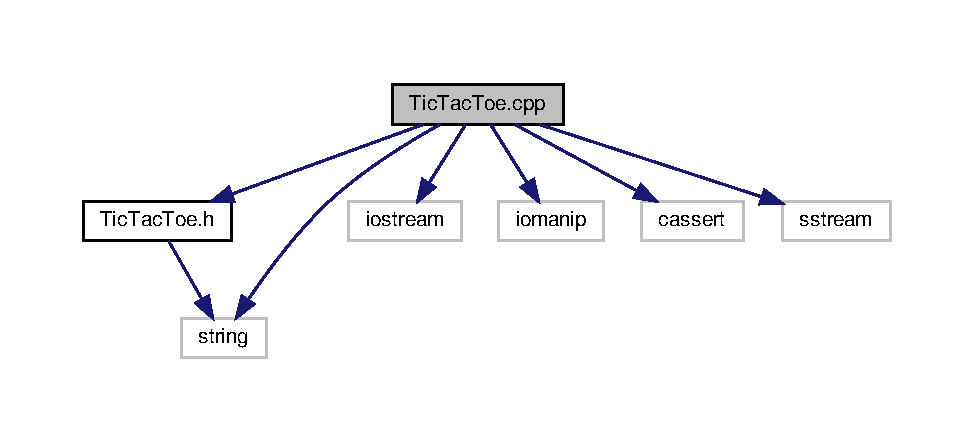
\includegraphics[width=350pt]{TicTacToe_8cpp__incl}
\end{center}
\end{figure}


\subsection{Detailed Description}
Created on\+: 2020-\/10-\/10 \begin{DoxyAuthor}{Author}
\+: Pascal Charpentier 
\end{DoxyAuthor}

%--- End generated contents ---

% Index
\backmatter
\newpage
\phantomsection
\clearemptydoublepage
\addcontentsline{toc}{chapter}{Index}
\printindex

\end{document}
